\documentclass[12pt,a4paper]{report}
% Paquetes básicos
\usepackage[utf8]{inputenc}
\usepackage[T1]{fontenc}
\usepackage[spanish]{babel}
\usepackage{graphicx}
\usepackage{geometry}
\usepackage{hyperref}
\usepackage{xcolor}
\usepackage{enumitem}
\geometry{margin=2.5cm}

% Configuración de hipervínculos
\hypersetup{
    colorlinks=true,
    linkcolor=blue,
    filecolor=magenta,
    urlcolor=cyan,
}

% Información del documento
\title{\textbf{Informe de Desarrollo}\\[0.5cm]{\Large Herramienta Diagnóstica para Transparencia, Participación y Evaluación Ambiental}\\[0.5cm]{\normalsize Ministerio de Ambiente y Desarrollo Sostenible de Colombia}}
\author{Diego Mauricio Pardo Cabrera}
\date{\today}

\begin{document}
\maketitle
\tableofcontents
\newpage

%--------------------------------------------------
\chapter{Introducción}
La \textbf{HerramientaEscazú} es una aplicación web desarrollada para el Ministerio de Ambiente y Desarrollo Sostenible de Colombia con el propósito de apoyar a las entidades territoriales colombianas en la identificación de oportunidades de mejora frente a los compromisos de transparencia, participación y evaluación ambiental establecidos en el \textit{Acuerdo de Escazú}. Este acuerdo regional, firmado en marzo de 2018 en Escazú (Costa Rica), representa el primer tratado ambiental de América Latina y el Caribe que busca garantizar la implementación plena y efectiva de los derechos de acceso a la información ambiental, participación pública en los procesos de toma de decisiones y acceso a la justicia en asuntos ambientales.

Este informe describe detalladamente cada una de las funcionalidades implementadas, la arquitectura técnica adoptada, y los procesos de desarrollo que han permitido crear una herramienta integral de autodiagnóstico institucional adaptada específicamente al contexto colombiano. La aplicación no solo permite evaluar el estado actual de cumplimiento de las entidades territoriales en Colombia, sino que también ofrece recomendaciones específicas para avanzar en la implementación de los principios del acuerdo de acuerdo con el marco normativo y contexto institucional nacional.

%--------------------------------------------------
\chapter{Arquitectura General}
La aplicación se ha desarrollado siguiendo principios de arquitectura moderna, con énfasis en escalabilidad, mantenibilidad y facilidad de uso. Se compone de:

\begin{itemize}[leftmargin=*]
    \item \textbf{Frontend}: construido con Next.js 14 y TypeScript, emplea un enfoque de componentes reutilizables y diseño totalmente responsivo mediante Tailwind CSS. La interfaz se adapta automáticamente a diferentes dispositivos, desde móviles hasta pantallas de escritorio de gran tamaño.
    
    \item \textbf{Backend}: implementado como una API REST (rutas \texttt{app/api/*}) que gestiona autenticación, preguntas, módulos, respuestas y evaluaciones. Utiliza el enrutador de aplicaciones de Next.js (App Router) para una gestión eficiente de las solicitudes.
    
    \item \textbf{Base de datos}: persistencia de la información mediante Prisma ORM, ofreciendo un mapeo seguro y tipado entre los objetos de la aplicación y las tablas de la base de datos PostgreSQL. El esquema está optimizado para consultas rápidas y relaciones complejas entre entidades.
    
    \item \textbf{Capa de autenticación}: sistema basado en tokens JWT para garantizar la seguridad de las operaciones administrativas, con verificación en cada solicitud a endpoints protegidos.
\end{itemize}

La arquitectura sigue el patrón Modelo-Vista-Controlador (MVC), separando claramente la lógica de negocio, la interfaz de usuario y el control de flujo de la aplicación.

%--------------------------------------------------
\chapter{Tecnologías Utilizadas}
El proyecto implementa un stack tecnológico moderno y robusto:

\begin{itemize}[leftmargin=*]
    \item \textbf{Next.js 14}: framework React con renderizado híbrido (servidor/cliente) que optimiza el rendimiento y SEO.
    
    \item \textbf{React 18 y TypeScript}: proporcionan un desarrollo basado en componentes con tipado estático para reducir errores y mejorar la mantenibilidad.
    
    \item \textbf{Tailwind CSS y Shadcn UI}: sistema de diseño utilitario combinado con componentes accesibles y personalizables que aceleran el desarrollo de interfaces coherentes.
    
    \item \textbf{Prisma ORM}: abstracción de base de datos con generación de clientes tipados que eliminan la necesidad de escribir SQL manual y reducen riesgos de inyección.
    
    \item \textbf{PostgreSQL}: sistema de gestión de bases de datos relacional con soporte para operaciones complejas y garantía de integridad de datos.
    
    \item \textbf{JWT (JSON Web Tokens)}: mecanismo de autenticación sin estado que facilita la validación de identidad en operaciones administrativas.
    
    \item \textbf{Docker}: contenedorización para garantizar consistencia entre entornos de desarrollo y producción.
    
    \item \textbf{ESLint y Prettier}: herramientas de análisis estático y formateo de código que aseguran la calidad y consistencia del código fuente.
\end{itemize}

%--------------------------------------------------
\chapter{Estructura del Proyecto}
El código fuente se organiza siguiendo las mejores prácticas de desarrollo de aplicaciones Next.js, con una estructura clara y modular:

\begin{itemize}[leftmargin=*]
    \item \texttt{app/}: implementa la estructura de rutas y páginas según el patrón de App Router de Next.js.
    \begin{itemize}
        \item \texttt{page.tsx}: página principal que muestra el formulario de inicio.
        \item \texttt{admin/}: rutas protegidas para el panel administrativo.
        \item \texttt{api/}: endpoints para operaciones CRUD y lógica de negocio.
    \end{itemize}
    
    \item \texttt{components/}: componentes reutilizables organizados por dominio funcional.
    \begin{itemize}
        \item \texttt{admin/}: componentes exclusivos del panel administrativo.
        \item \texttt{ui/}: componentes de interfaz genéricos basados en Shadcn UI.
        \item Componentes específicos como \texttt{quiz-layout.tsx}, \texttt{question-card.tsx}, etc.
    \end{itemize}
    
    \item \texttt{lib/}: utilidades, lógica de puntuación, helpers y conexión a la base de datos.
    \begin{itemize}
        \item \texttt{database.ts}: configuración y conexión a la base de datos.
        \item \texttt{scoring.ts}: algoritmos de cálculo y evaluación de puntajes.
        \item \texttt{utils.ts}: funciones auxiliares utilizadas en toda la aplicación.
    \end{itemize}
    
    \item \texttt{hooks/}: hooks personalizados de React para lógica reutilizable.
    \item \texttt{public/}: activos estáticos como imágenes y archivos de fuentes.
    \item \texttt{styles/}: estilos globales y configuración de Tailwind CSS.
\end{itemize}

Esta organización facilita la localización de código, promueve la reutilización y permite un desarrollo paralelo eficiente por parte del equipo.

%--------------------------------------------------
\chapter{Funcionalidades Principales}

\section{Formulario de Caracterización del Evaluador}
La experiencia del usuario comienza con un formulario de caracterización que recopila información esencial sobre el evaluador y su entidad. Este paso es fundamental para contextualizar los resultados y permitir análisis posteriores por segmentos.

\begin{figure}[h]
    \centering
    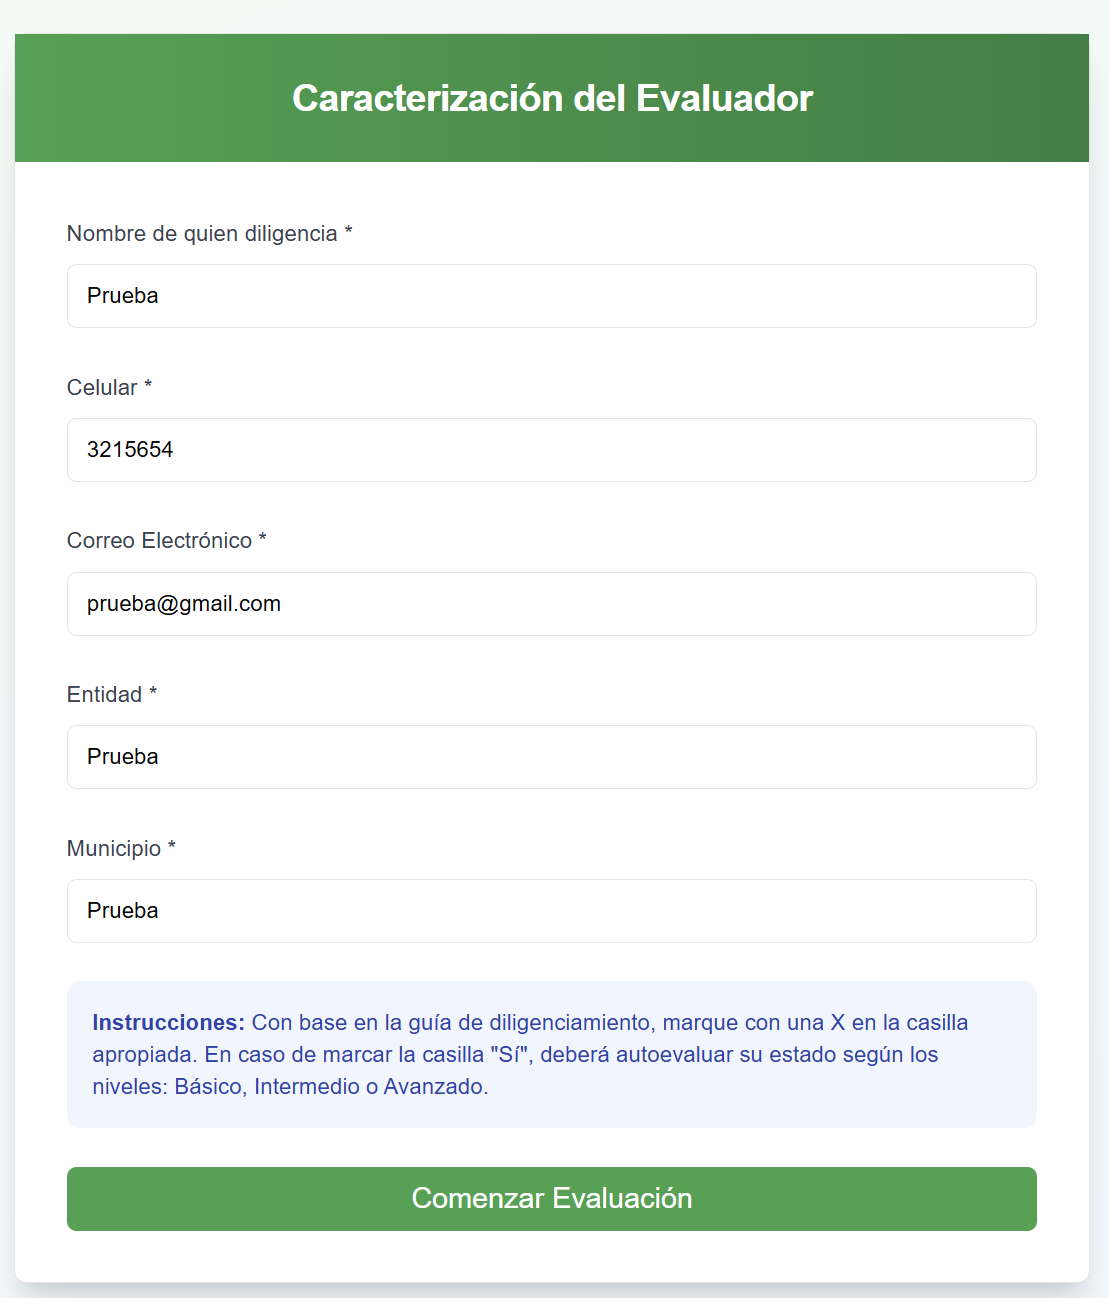
\includegraphics[width=0.85\textwidth]{Captura de pantalla 2025-06-26 121654.png}
    \caption{Formulario de caracterización del evaluador}
\end{figure}

El formulario incluye:
\begin{itemize}[leftmargin=*]
    \item \textbf{Datos personales}: nombre completo, correo electrónico y número de contacto del funcionario que realiza la evaluación.
    \item \textbf{Información institucional}: nombre de la entidad territorial, departamento y municipio de Colombia.
    \item \textbf{Datos de caracterización}: tipo de entidad (alcaldía, gobernación, corporación autónoma regional, etc.), rol o cargo del evaluador, y área o dependencia específica dentro del sistema administrativo colombiano.
\end{itemize}

La interfaz implementa validación en tiempo real con mensajes de error contextuales que guían al usuario en caso de datos incorrectos o faltantes. El diseño minimalista con campos claramente etiquetados facilita la experiencia del usuario y reduce la fricción inicial. Los catálogos de departamentos y municipios están adaptados específicamente a la división político-administrativa de Colombia.

\section{Módulo de Evaluación Dinámica}
El núcleo funcional de la aplicación es el sistema de evaluación dinámica, que presenta secuencialmente las preguntas organizadas por módulos temáticos. Cada evaluación consta de 37 preguntas distribuidas en tres módulos principales correspondientes a los pilares del Acuerdo de Escazú.

\begin{figure}[h]
    \centering
    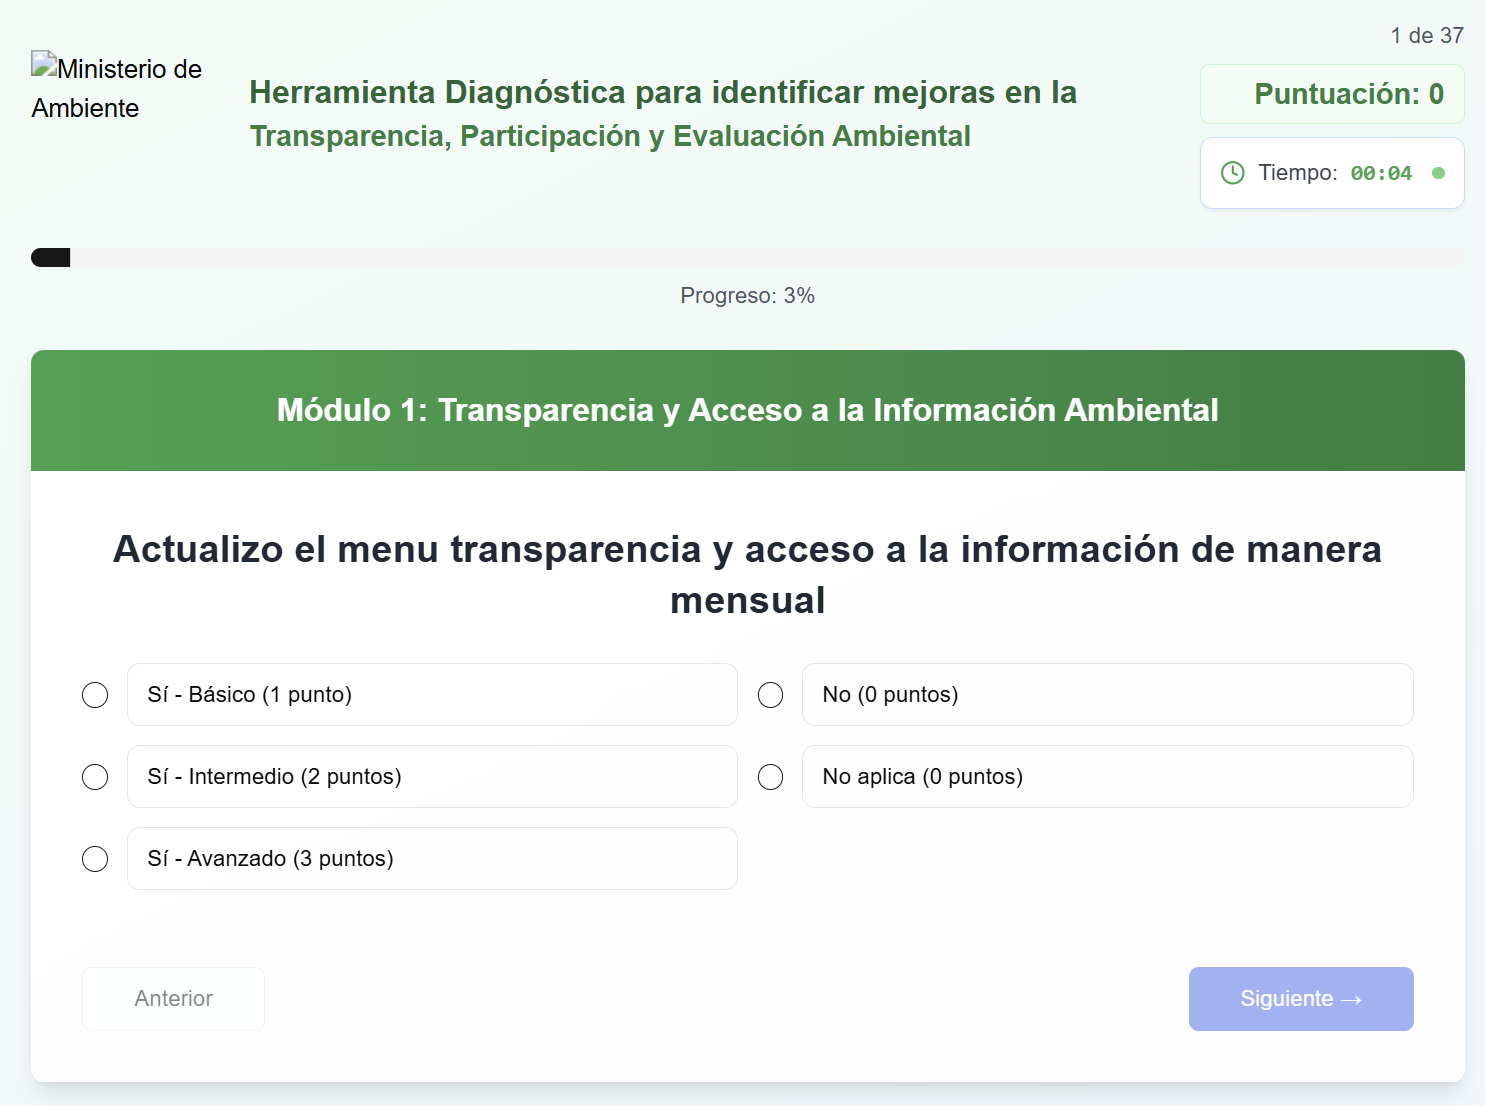
\includegraphics[width=0.85\textwidth]{Captura de pantalla 2025-06-26 121706.png}
    \caption{Interfaz de evaluación mostrando la primera pregunta del Módulo 1}
\end{figure}

La interfaz de evaluación incluye:
\begin{itemize}[leftmargin=*]
    \item \textbf{Barra superior}: muestra el módulo actual, indicador de progreso visual (barra azul) y cronómetro para medir el tiempo invertido en la evaluación.
    \item \textbf{Tarjeta de pregunta}: presenta cada pregunta con su texto completo, contexto adicional cuando es necesario y opciones de respuesta específicas.
    \item \textbf{Opciones de respuesta}: cada pregunta ofrece alternativas apropiadas a su naturaleza. En la imagen se observan opciones de selección única con niveles de implementación (No implementado, Implementado parcialmente, Implementado totalmente).
    \item \textbf{Sistema de puntuación}: cada opción muestra claramente el puntaje asociado (0, 1 o 2 puntos en este ejemplo), permitiendo al usuario comprender cómo sus respuestas impactan en la evaluación final.
    \item \textbf{Navegación}: botones "Anterior" y "Siguiente" para moverse entre preguntas, con lógica que previene avanzar si no se ha respondido la pregunta actual.
\end{itemize}

El sistema admite distintos tipos de preguntas, adaptando la interfaz según sea necesario. Algunas preguntas solicitan respuestas binarias (Sí/No) mientras que otras permiten elegir entre niveles de implementación o conformidad.

\begin{figure}[h]
    \centering
    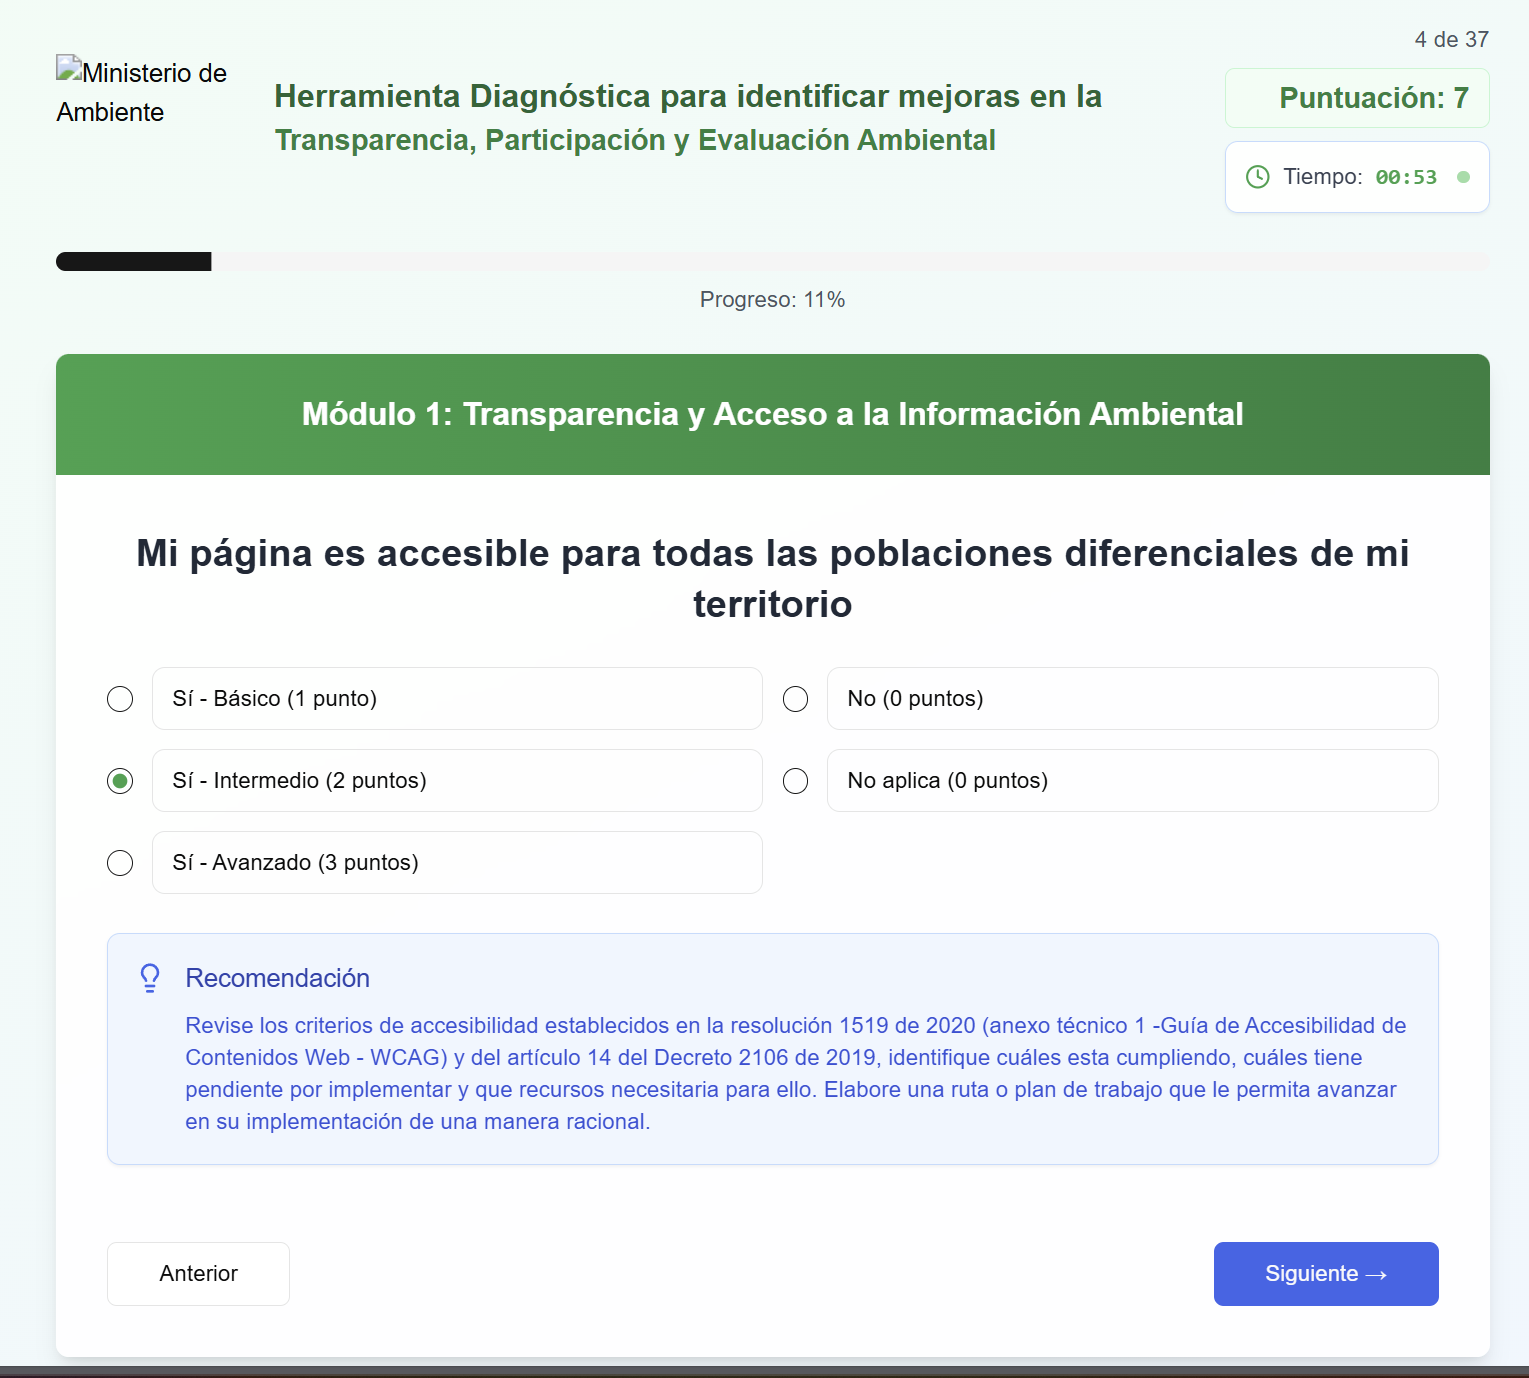
\includegraphics[width=0.85\textwidth]{Captura de pantalla 2025-06-26 121754.png}
    \caption{Pregunta con campo obligatorio de justificación y opciones de respuesta binaria}
    \label{fig:justificacion}
\end{figure}

Como se observa en la Figura~\ref{fig:justificacion}, ciertos tipos de pregunta requieren justificación textual. En este caso:
\begin{itemize}[leftmargin=*]
    \item La pregunta solicita información sobre la existencia de espacios designados para audiencias públicas ambientales.
    \item El usuario debe seleccionar "Sí" o "No" como respuesta principal.
    \item El campo de justificación se convierte en obligatorio, solicitando detalles específicos que respalden la respuesta seleccionada.
    \item Un contador de caracteres ayuda al usuario a mantener su justificación dentro del límite establecido.
    \item El formato de la tarjeta mantiene una estructura coherente con el resto de la evaluación para facilitar la navegación.
\end{itemize}

La justificación es especialmente importante para preguntas de tipo cualitativo, ya que permite contextualizar las respuestas y proporcionar evidencia que respalde la autoevaluación realizada por la entidad.

\section{Motor de Recomendaciones}
Una característica distintiva de la herramienta es su capacidad para ofrecer retroalimentación inmediata basada en las respuestas del usuario. El motor de recomendaciones analiza cada respuesta y presenta sugerencias contextualizadas para mejorar el desempeño en el área específica.

\begin{figure}[h]
    \centering
    
\includegraphics[width=0.85\textwidth]{Captura de pantalla 2025-06-26 121833.png}
    \caption{Panel de recomendación automática generada en respuesta a la selección del usuario}
    \label{fig:recomendacion}
\end{figure}

La Figura~\ref{fig:recomendacion} muestra cómo funciona el motor de recomendaciones:
\begin{itemize}[leftmargin=*]
    \item \textbf{Activación contextual}: la recomendación aparece inmediatamente después de que el usuario selecciona una respuesta, sin necesidad de esperar a finalizar toda la evaluación.
    \item \textbf{Contenido específico}: la recomendación mostrada está directamente relacionada con la opción seleccionada. En este ejemplo, se sugieren acciones específicas para mejorar la disponibilidad de información ambiental en situaciones de emergencia.
    \item \textbf{Formato visual distintivo}: las recomendaciones se presentan en un panel amarillo con formato destacado para diferenciarlas del resto del contenido y captar la atención del usuario.
    \item \textbf{Información accionable}: cada recomendación incluye pasos concretos que la entidad puede implementar para mejorar su desempeño, no sólo identificando deficiencias sino ofreciendo soluciones prácticas.
\end{itemize}

Esta funcionalidad convierte la herramienta de un simple sistema de evaluación a una plataforma educativa que orienta a las entidades en su proceso de mejora continua. Las recomendaciones se almacenan junto con las respuestas para incluirlas posteriormente en el informe final de resultados.

\section{Cálculo de Puntaje y Clasificación}
El corazón matemático de la aplicación reside en su algoritmo de puntuación implementado en el archivo \texttt{lib/scoring.ts}. Este sistema realiza las siguientes operaciones:

\begin{itemize}[leftmargin=*]
    \item \textbf{Suma ponderada}: cada respuesta tiene un peso específico según su relevancia dentro del marco del Acuerdo de Escazú.
    \item \textbf{Cálculo porcentual}: el total acumulado se convierte a un porcentaje sobre el máximo posible, considerando solo las preguntas aplicables a la entidad particular.
    \item \textbf{Clasificación por umbrales}: el porcentaje obtenido se compara con umbrales configurables para asignar una categoría:
    \begin{itemize}
        \item \textit{Básico}: 0-40\% del puntaje máximo
        \item \textit{Intermedio}: 41-75\% del puntaje máximo
        \item \textit{Avanzado}: 76-100\% del puntaje máximo
    \end{itemize}
    \item \textbf{Desglose por módulos}: además del puntaje global, se calculan subtotales para cada uno de los tres módulos, permitiendo identificar áreas específicas de fortaleza y oportunidad.
\end{itemize}

El algoritmo considera la opción "No aplica" de manera especial, ajustando el denominador para evitar penalizar a entidades por aspectos que no corresponden a su naturaleza o competencias legales.

\section{Resultados Detallados}
Al finalizar la evaluación, el sistema genera automáticamente un informe completo de resultados que sintetiza el desempeño de la entidad y proporciona una hoja de ruta para la mejora.

\begin{figure}[h]
    \centering
    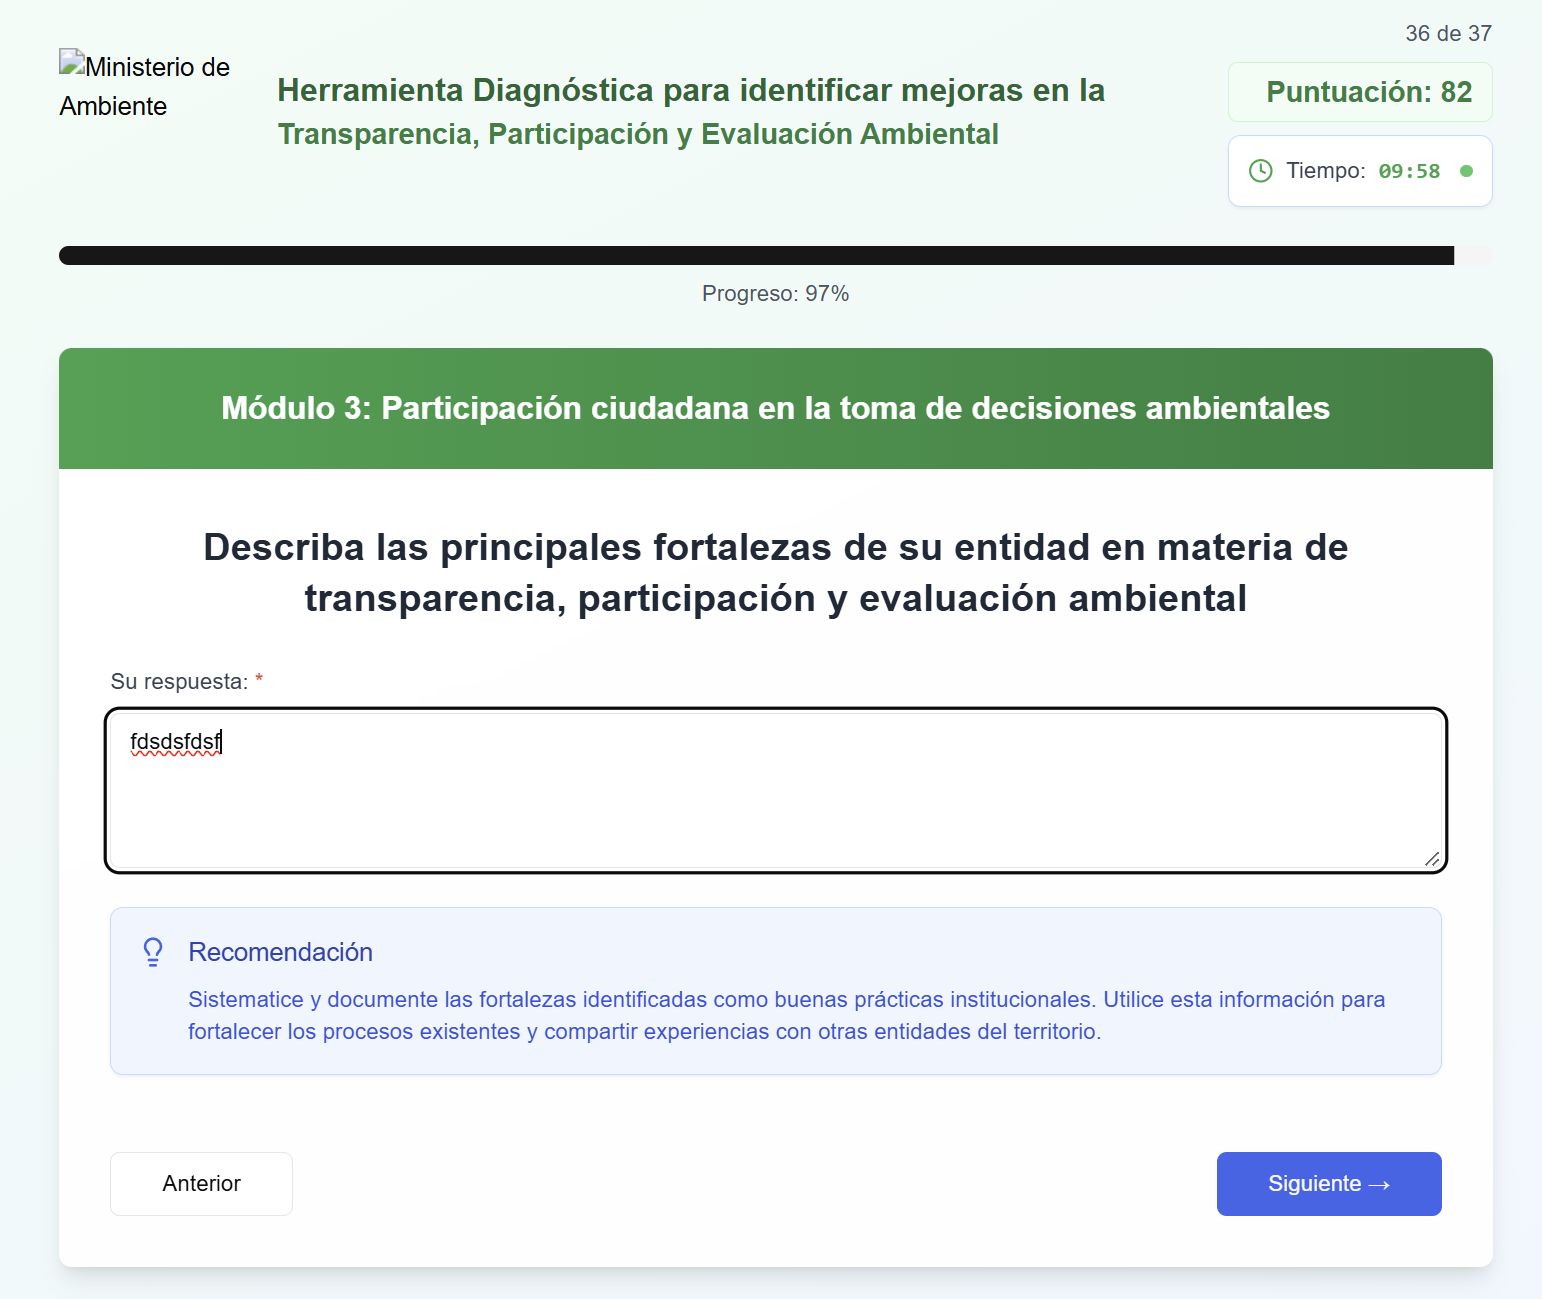
\includegraphics[width=0.85\textwidth]{Captura de pantalla 2025-06-26 122659.png}
    \caption{Pantalla de resultados finales mostrando puntaje, clasificación y desglose por módulos}
\end{figure}

La interfaz de resultados incluye:
\begin{itemize}[leftmargin=*]
    \item \textbf{Encabezado}: muestra el nombre de la entidad evaluada y la fecha de realización.
    \item \textbf{Puntaje global}: visualización prominente del porcentaje total obtenido (74\% en el ejemplo) y la clasificación resultante ("Intermedio").
    \item \textbf{Representación gráfica}: un medidor semicircular que comunica visualmente el nivel alcanzado, con código de colores intuitivo (verde para avanzado, amarillo para intermedio, rojo para básico).
    \item \textbf{Desglose por módulos}: gráficas de barras que muestran el desempeño relativo en cada uno de los tres módulos temáticos, permitiendo identificar áreas de fortaleza y oportunidad.
    \item \textbf{Resumen de respuestas}: listado expandible con todas las preguntas, las respuestas seleccionadas, justificaciones proporcionadas y recomendaciones específicas.
    \item \textbf{Opciones de exportación}: funcionalidad para descargar los resultados completos en formato PDF o compartirlos mediante enlace directo.
\end{itemize}

Esta visualización integral permite a los tomadores de decisiones comprender rápidamente el estado general de cumplimiento y los aspectos específicos que requieren atención prioritaria.

%--------------------------------------------------
\chapter{Panel de Administración}
El sistema incluye un robusto panel administrativo diseñado para la gestión integral del contenido y el monitoreo de las evaluaciones realizadas. El acceso está protegido mediante credenciales específicas y autenticación basada en tokens JWT.

\section{Dashboard}
La página principal del panel administrativo presenta una visión general del sistema, con métricas clave y visualizaciones que facilitan la toma de decisiones.

\begin{figure}[h]
    \centering
    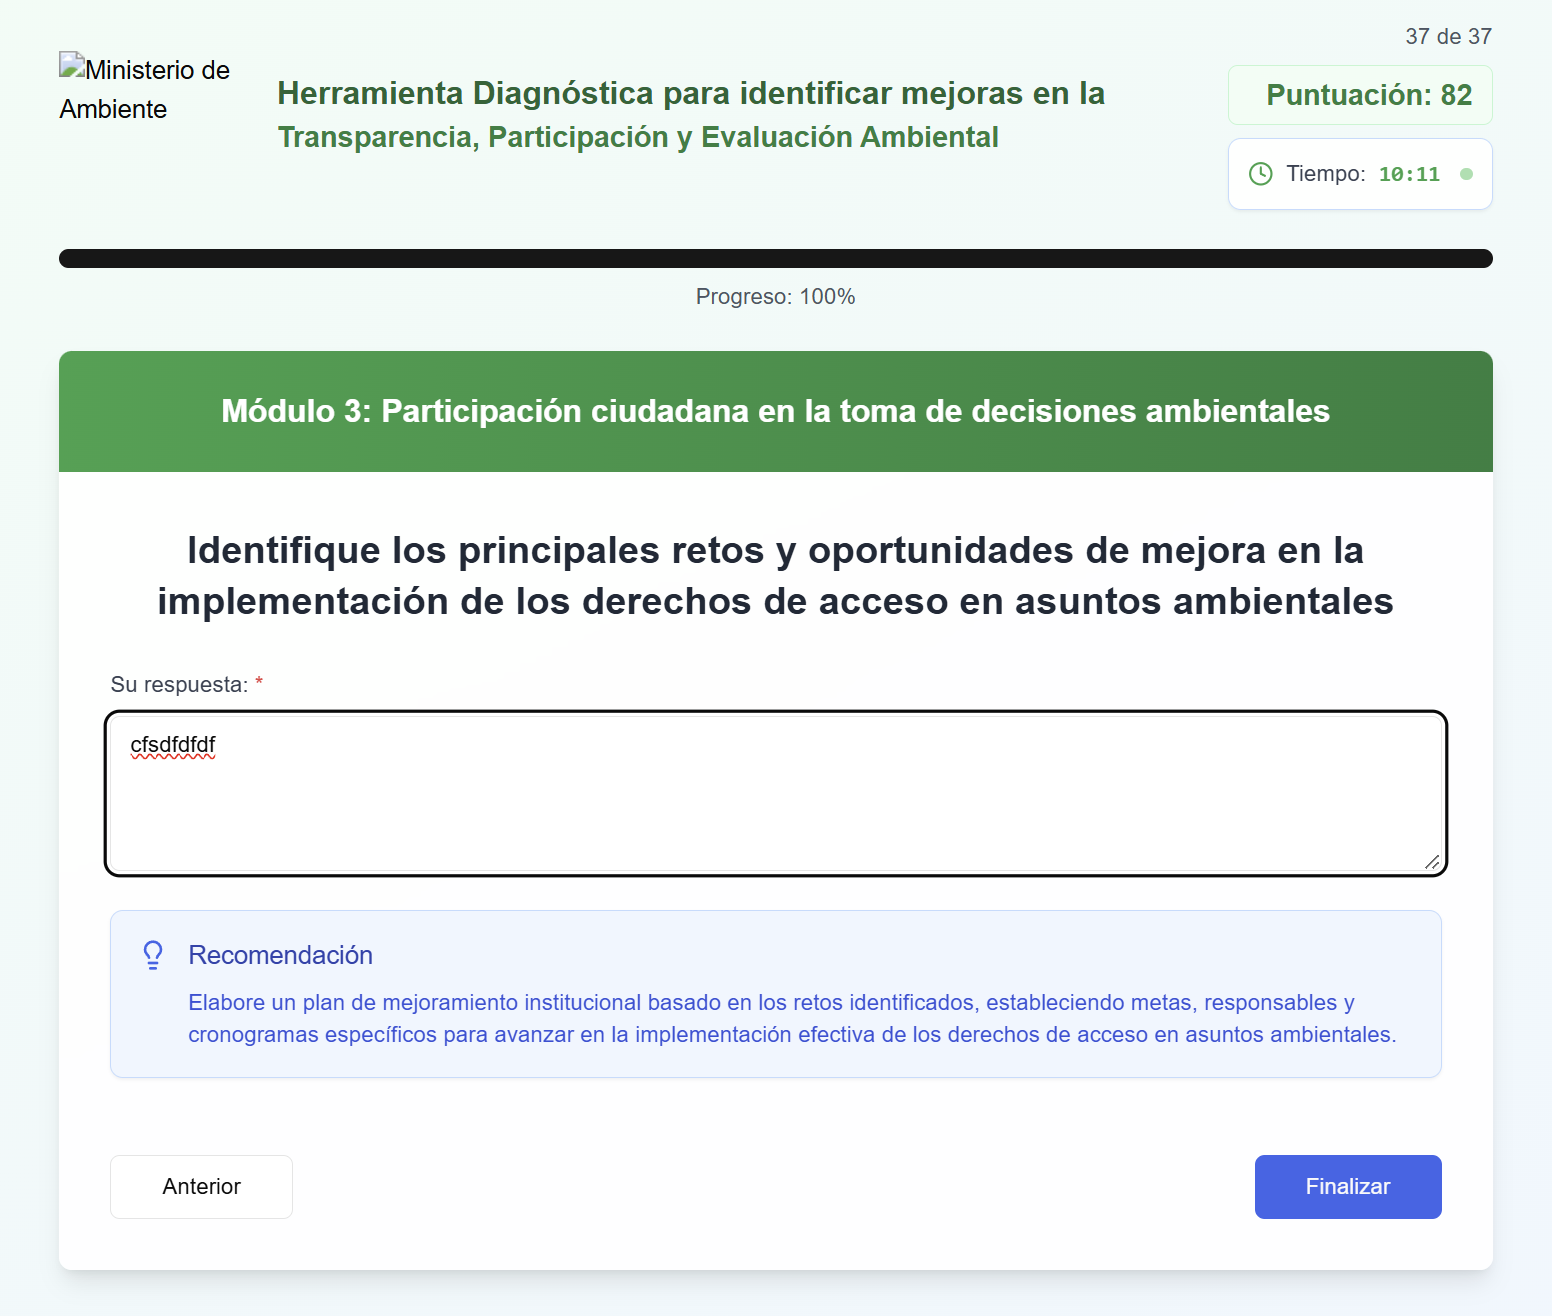
\includegraphics[width=0.85\textwidth]{Captura de pantalla 2025-06-26 122710.png}
    \caption{Dashboard administrativo con métricas de uso y visualizaciones de datos}
\end{figure}

El dashboard incluye:
\begin{itemize}[leftmargin=*]
    \item \textbf{Tarjetas de resumen}: muestran el número total de evaluaciones completadas, preguntas activas en el sistema, módulos configurados y usuarios administrativos.
    \item \textbf{Distribución por clasificación}: gráfico circular que visualiza la proporción de entidades en cada categoría (Básico, Intermedio, Avanzado), ofreciendo una perspectiva estadística del estado general de cumplimiento.
    \item \textbf{Tendencia temporal}: gráfico lineal que muestra la evolución de las evaluaciones completadas a lo largo del tiempo, permitiendo identificar patrones de uso y picos de actividad.
    \item \textbf{Mapa de calor por departamentos}: visualización geográfica que identifica las regiones de Colombia con mayor y menor participación en la evaluación, utilizando la división político-administrativa oficial del país.
    \item \textbf{Actividad reciente}: listado de las últimas evaluaciones completadas con enlaces directos para revisar los detalles específicos.
\end{itemize}

Esta interfaz está diseñada para que los administradores del Ministerio de Ambiente y Desarrollo Sostenible puedan monitorear el uso de la herramienta y obtener insights estratégicos sin necesidad de generar reportes manuales, facilitando así la toma de decisiones basadas en datos para la implementación del Acuerdo de Escazú en el territorio colombiano.

\section{Gestión de Preguntas}
El módulo de gestión de preguntas permite a los administradores mantener actualizado el banco de preguntas, adaptándolo a nuevas normativas o necesidades específicas de evaluación.

\begin{figure}[h]
    \centering
    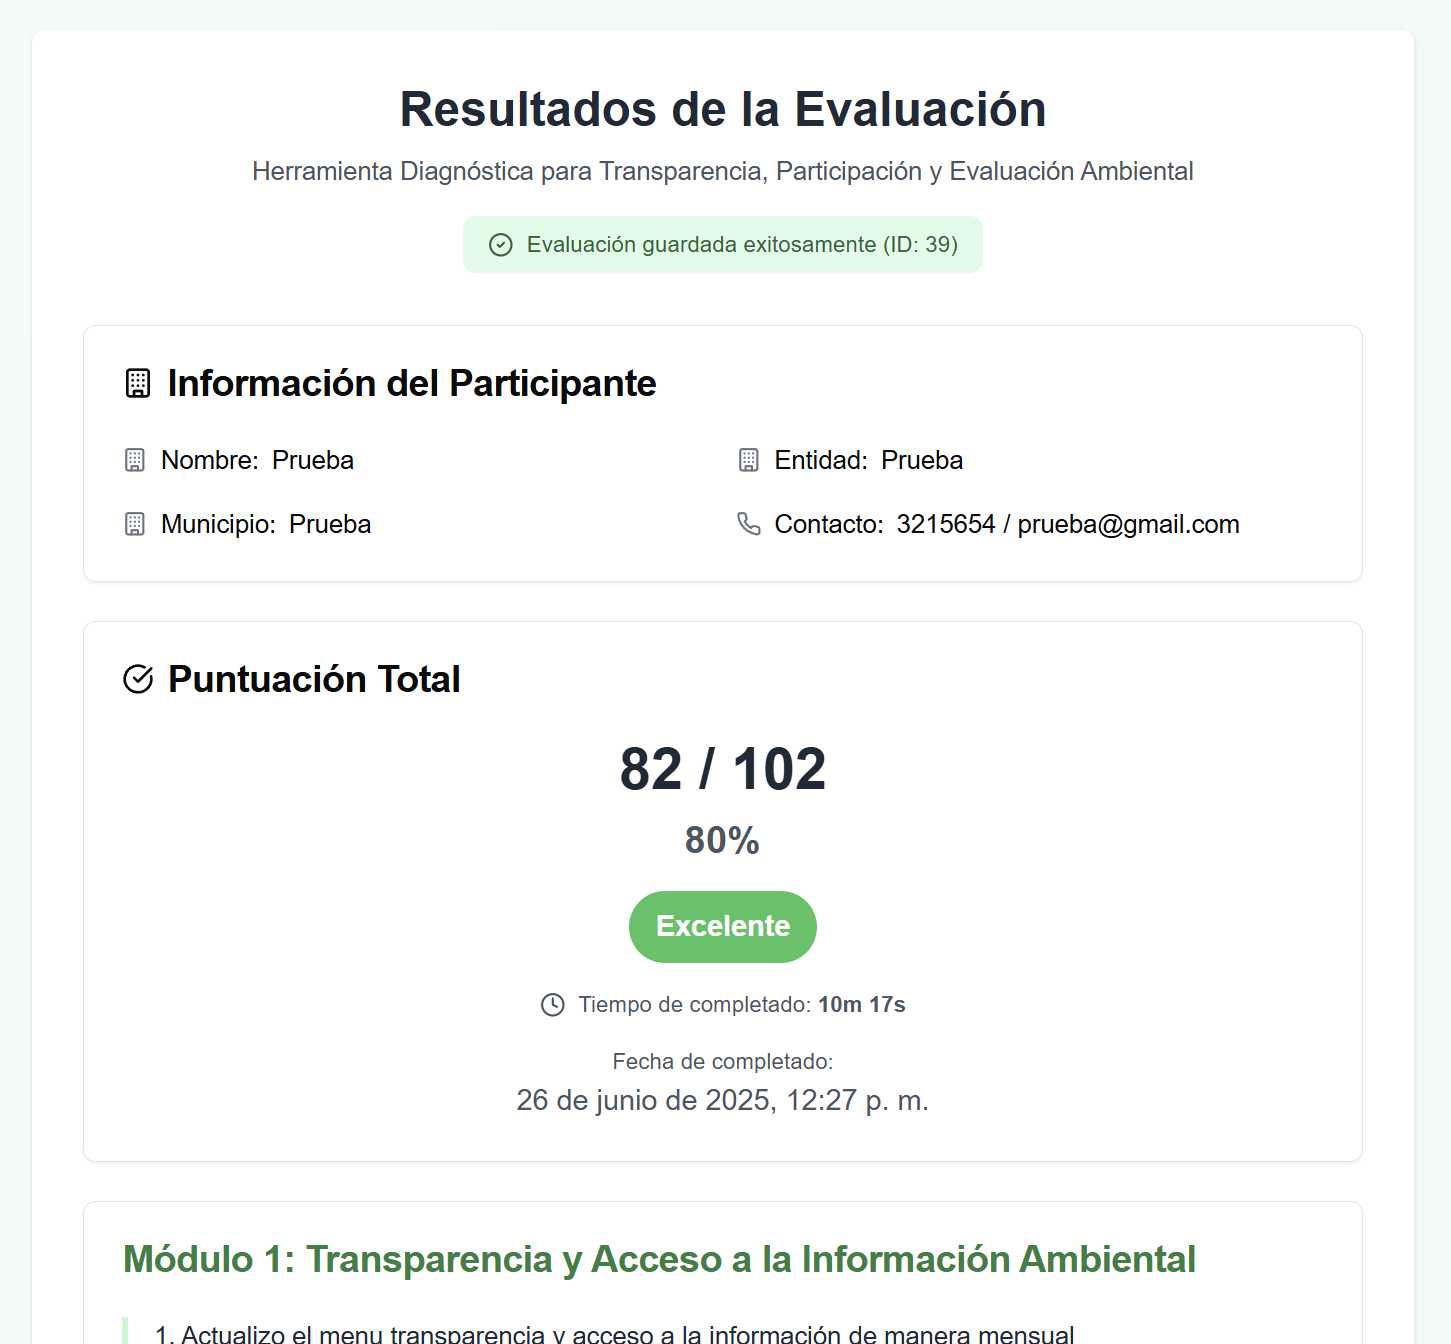
\includegraphics[width=0.85\textwidth]{Captura de pantalla 2025-06-26 122733.png}
    \caption{Interfaz de gestión de preguntas con listado, búsqueda y opciones de edición}
\end{figure}

La interfaz de gestión de preguntas ofrece:
\begin{itemize}[leftmargin=*]
    \item \textbf{Listado paginado}: muestra las preguntas existentes con su texto, módulo asociado y tipo de respuesta esperada.
    \item \textbf{Búsqueda y filtrado}: permite localizar rápidamente preguntas específicas por texto o módulo.
    \item \textbf{Formulario de creación/edición}: interfaz intuitiva para definir cada aspecto de una pregunta:
    \begin{itemize}
        \item Texto principal y descripción adicional
        \item Módulo al que pertenece y orden de aparición
        \item Tipo de respuesta (binaria, múltiple, con justificación)
        \item Puntaje asociado a cada opción de respuesta
        \item Recomendaciones específicas para cada posible respuesta
    \end{itemize}
    \item \textbf{Funcionalidad de arrastrar y soltar}: permite reordenar visualmente las preguntas dentro de cada módulo.
    \item \textbf{Vista previa}: muestra cómo se verá la pregunta en el formulario de evaluación antes de publicarla.
\end{itemize}

El sistema asegura la integridad referencial, garantizando que los cambios en las preguntas no afecten las evaluaciones históricas ya completadas, que mantienen una copia de la estructura de preguntas vigente al momento de su realización.

\section{Gestión de Módulos}
Los módulos temáticos organizan las preguntas en grupos coherentes, facilitando la navegación y comprensión del proceso de evaluación. El panel administrativo incluye herramientas específicas para su gestión.

\begin{figure}[h]
    \centering
    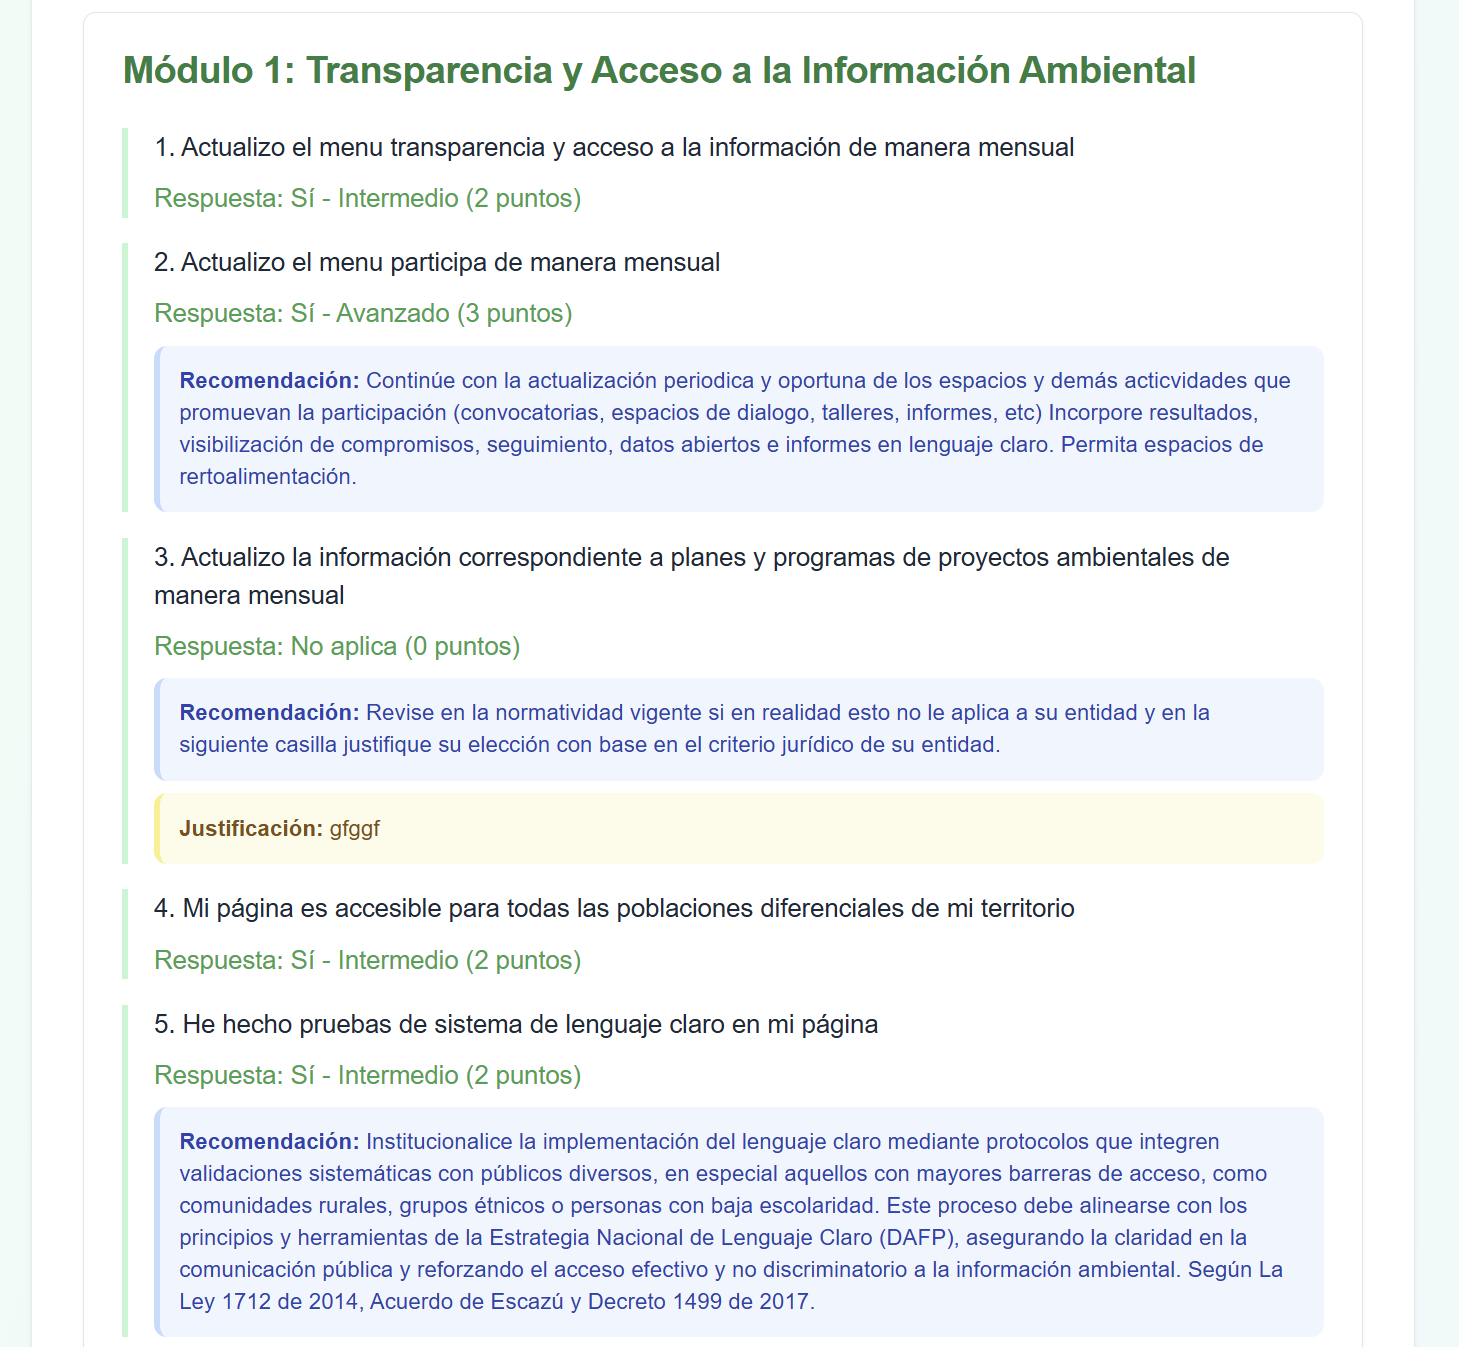
\includegraphics[width=0.85\textwidth]{Captura de pantalla 2025-06-26 122745.png}
    \caption{Interfaz de gestión de módulos temáticos con opciones de edición y estadísticas}
\end{figure}

La interfaz de gestión de módulos presenta:
\begin{itemize}[leftmargin=*]
    \item \textbf{Listado de módulos}: muestra los módulos existentes con su nombre, descripción breve y número de preguntas asociadas.
    \item \textbf{Formulario de creación/edición}: permite configurar cada módulo con:
    \begin{itemize}
        \item Título principal y descripción detallada
        \item Color distintivo para identificación visual
        \item Orden de aparición en la evaluación
        \item Peso relativo en el cálculo de la puntuación final (opcional)
    \end{itemize}
    \item \textbf{Estadísticas por módulo}: gráficos que muestran el desempeño promedio de las entidades evaluadas en cada módulo, identificando patrones y áreas de dificultad común.
    \item \textbf{Visualización de estructura}: diagrama que muestra la distribución de preguntas por módulo y las interrelaciones temáticas.
\end{itemize}

Esta organización modular facilita no solo la experiencia del usuario final, sino también la administración y análisis de resultados por áreas temáticas específicas.

\section{Gestión de Evaluaciones}
El seguimiento y análisis de las evaluaciones completadas es una funcionalidad clave para los administradores, permitiendo extraer conclusiones a nivel agregado y monitorear el progreso de entidades específicas.

\begin{figure}[h]
    \centering
    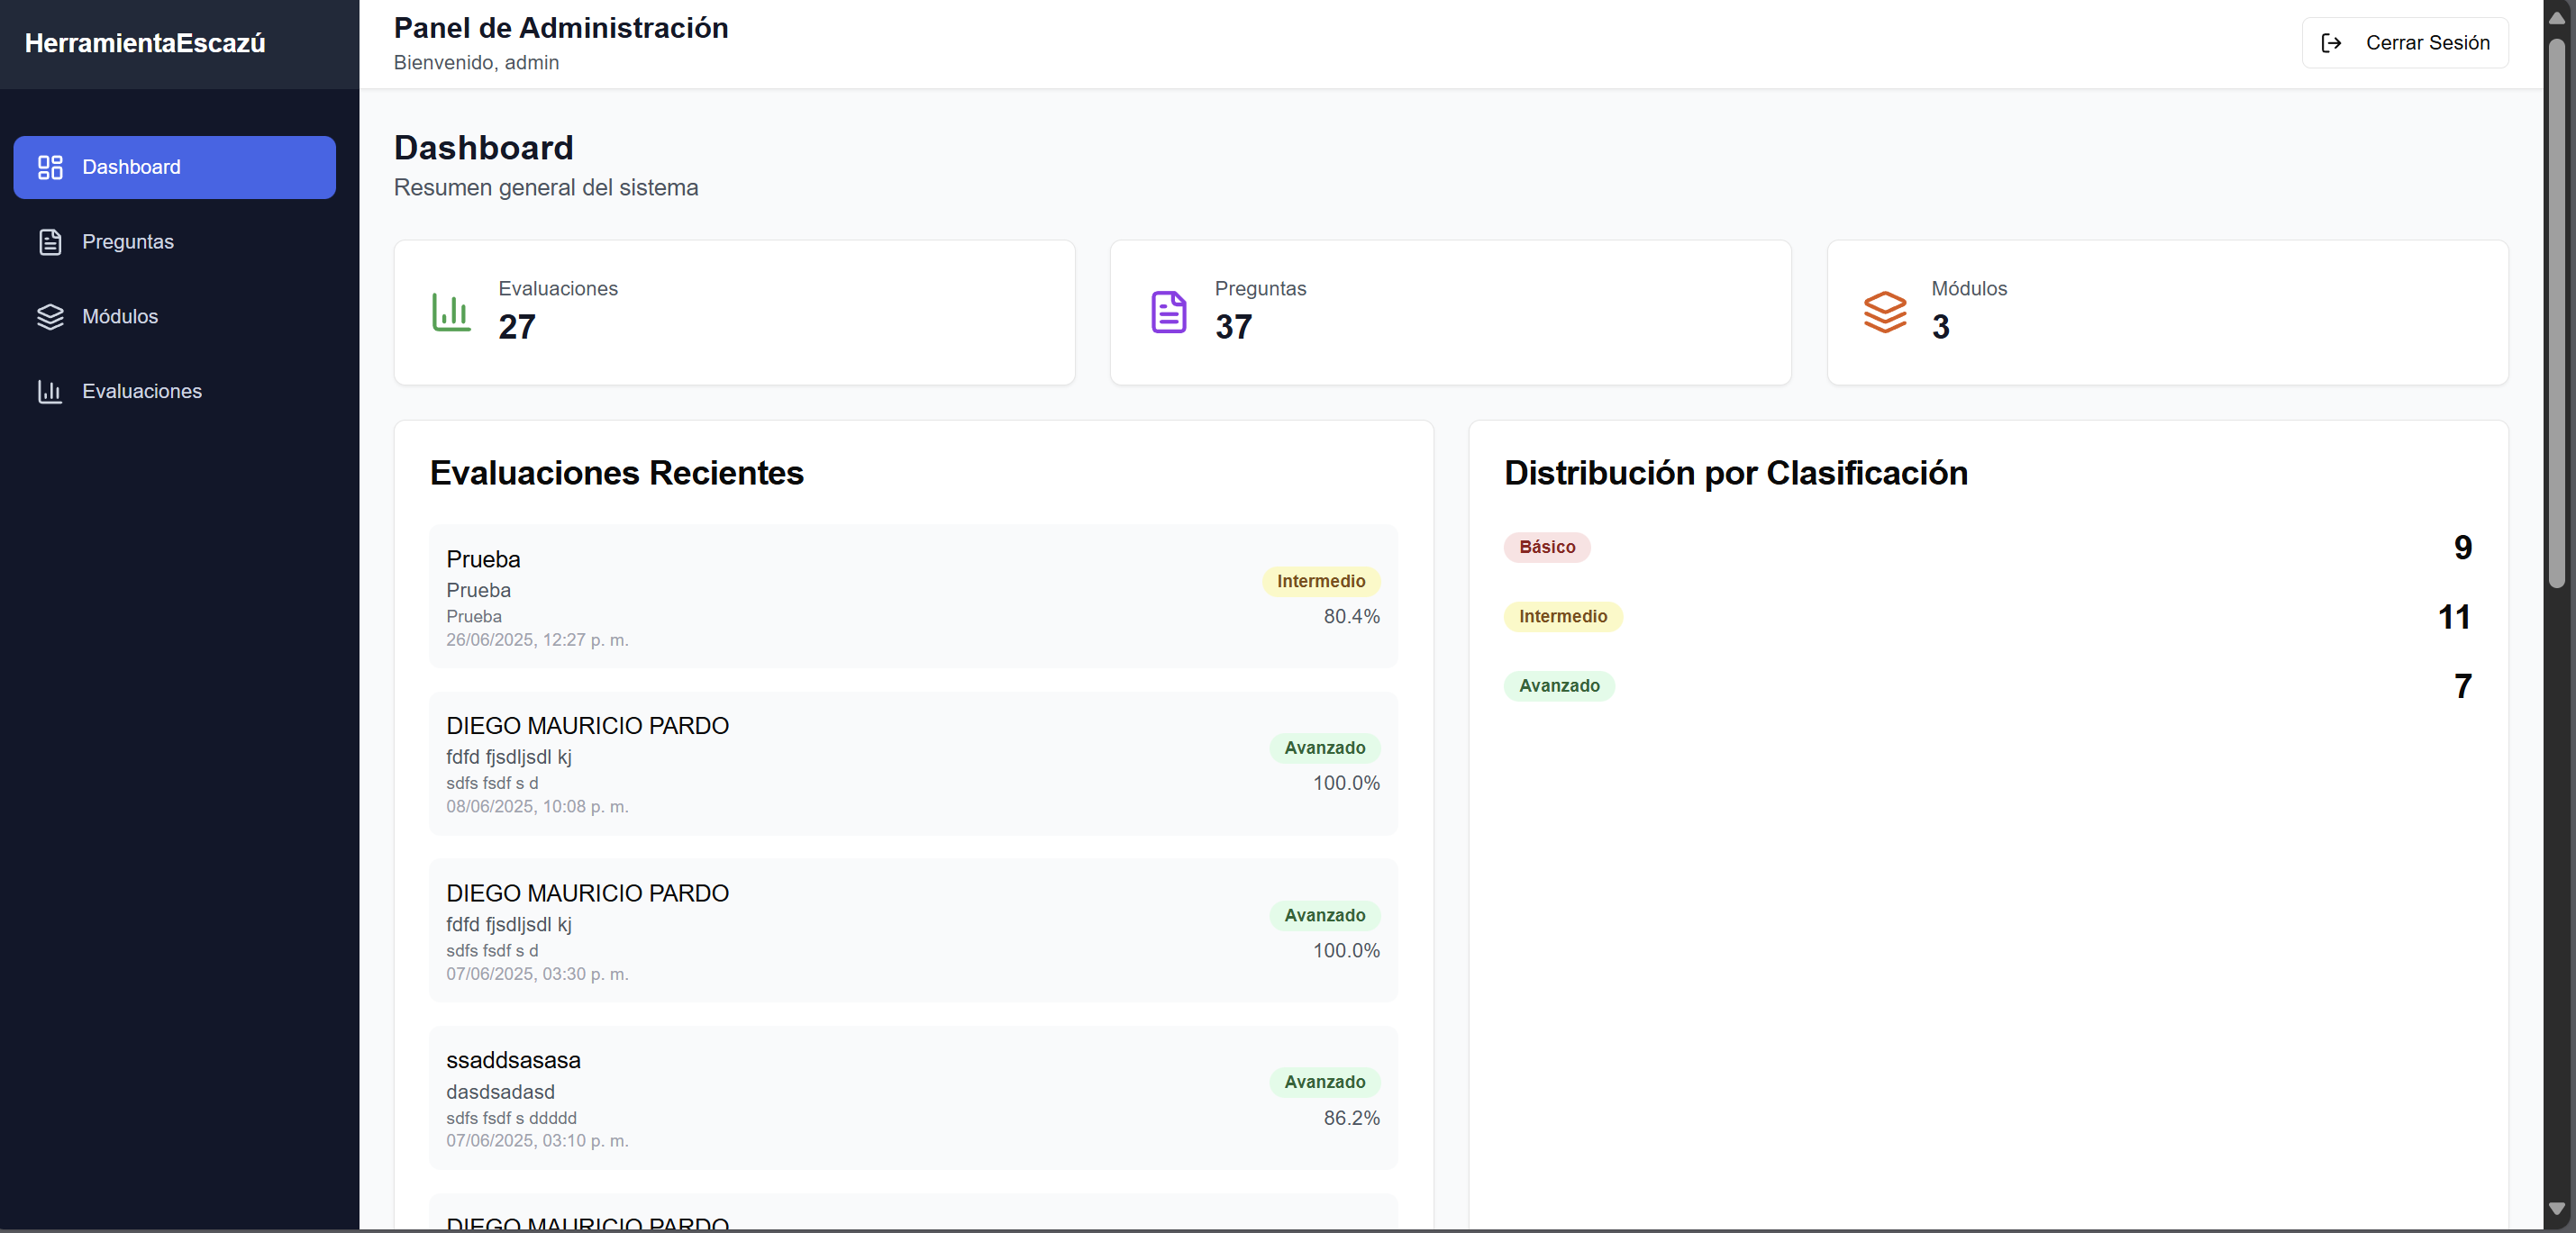
\includegraphics[width=0.85\textwidth]{Captura de pantalla 2025-06-26 122831.png}
    \caption{Panel de gestión de evaluaciones con opciones de filtrado y exportación de datos}
\end{figure}

La interfaz de gestión de evaluaciones incluye:
\begin{itemize}[leftmargin=*]
    \item \textbf{Tabla completa}: listado de todas las evaluaciones realizadas con información clave como entidad, fecha, puntaje, clasificación y tiempo de compleción.
    \item \textbf{Filtros avanzados}: permite segmentar las evaluaciones por:
    \begin{itemize}
        \item Rango de fechas
        \item Departamento o municipio de Colombia
        \item Tipo de entidad según la estructura administrativa colombiana
        \item Clasificación obtenida
        \item Módulos específicos con mayor o menor desempeño
    \end{itemize}
    \item \textbf{Vista detallada}: acceso a la información completa de cada evaluación, incluyendo todas las respuestas y justificaciones proporcionadas.
    \item \textbf{Exportación de datos}: funcionalidad para descargar los resultados en múltiples formatos:
    \begin{itemize}
        \item CSV para análisis en herramientas estadísticas
        \item Excel para reportes internos del Ministerio
        \item PDF para presentaciones oficiales ante entidades nacionales
    \end{itemize}
    \item \textbf{Análisis comparativo}: herramienta para contrastar evaluaciones de diferentes periodos o entidades similares, visualizando avances o retrocesos en la implementación del Acuerdo de Escazú en Colombia.
\end{itemize}

Esta funcionalidad permite a los administradores del Ministerio generar informes agregados que pueden informar políticas públicas ambientales, identificar necesidades de capacitación en las diferentes regiones del país o resaltar casos de éxito para replicación en otros territorios colombianos.

%--------------------------------------------------
\chapter{Seguridad y Autenticación}
La seguridad es un aspecto fundamental de la aplicación, especialmente considerando que maneja datos institucionales sensibles y permite configuraciones que afectan la evaluación de entidades públicas.

La autenticación se implementa mediante JSON Web Tokens (JWT) siguiendo las mejores prácticas:
\begin{itemize}[leftmargin=*]
    \item \textbf{Autenticación basada en credenciales}: sistema de usuario/contraseña con políticas de complejidad y caducidad.
    \item \textbf{Tokens de sesión}: generados con expiración configurable (por defecto 24 horas) y firmados con clave secreta.
    \item \textbf{Verificación por ruta}: middleware que valida los tokens antes de permitir acceso a cualquier endpoint administrativo.
    \item \textbf{Protección CSRF}: implementación de tokens anti-falsificación para prevenir ataques de solicitud cruzada.
    \item \textbf{Cifrado TLS}: toda la comunicación se realiza sobre HTTPS para prevenir interceptación de credenciales.
    \item \textbf{Auditoría de acciones}: registro detallado de operaciones administrativas para trazabilidad.
\end{itemize}

Adicionalmente, la base de datos implementa cifrado para campos sensibles y la aplicación aplica principios de privilegio mínimo, exponiendo solo la información necesaria para cada tipo de usuario.

%--------------------------------------------------
\chapter{Despliegue y Entorno}
La aplicación está diseñada para facilitar su despliegue en la infraestructura tecnológica del Ministerio de Ambiente y Desarrollo Sostenible de Colombia.

\begin{itemize}[leftmargin=*]
    \item \textbf{Contenedorización}: la aplicación se distribuye como contenedores Docker interconectados:
    \begin{itemize}
        \item Contenedor de aplicación Next.js (frontend + API)
        \item Contenedor de base de datos PostgreSQL
        \item Contenedor opcional de caché Redis para optimización
    \end{itemize}
    
    \item \textbf{Configuración mediante variables de entorno}: parámetros como credenciales de base de datos, URL de la aplicación y claves secretas se configuran mediante variables de entorno, siguiendo las mejores prácticas de 12-factor app y las directrices de seguridad del Ministerio.
    
    \item \textbf{Scripts de inicialización}: incluye migraciones automáticas de base de datos y carga inicial de datos maestros (módulos y preguntas base) adaptados al contexto institucional colombiano.
    
    \item \textbf{Monitoreo integrado}: exporta métricas de rendimiento y uso para integración con los sistemas de monitoreo existentes en la infraestructura tecnológica del Ministerio.
    
    \item \textbf{Documentación detallada}: guías paso a paso para despliegue específicamente orientadas al entorno tecnológico del Ministerio de Ambiente:
    \begin{itemize}
        \item Despliegue en servidores del Ministerio
        \item Integración con directorio activo institucional
        \item Configuración de copias de seguridad según protocolos del Ministerio
        \item Procedimientos de actualización y mantenimiento
    \end{itemize}
\end{itemize}

El proceso de CI/CD está configurado para realizar pruebas automáticas y generar nuevas versiones de contenedores con cada cambio aprobado, garantizando la estabilidad y calidad del sistema según los estándares del gobierno digital colombiano.

%--------------------------------------------------
\chapter{Conclusiones y Trabajo Futuro}
La \textbf{HerramientaEscazú} representa una solución integral desarrollada específicamente para el Ministerio de Ambiente y Desarrollo Sostenible de Colombia, con el fin de evaluar y mejorar el cumplimiento de los compromisos establecidos en el Acuerdo de Escazú en el territorio colombiano. Su diseño modular, interfaz intuitiva y panel administrativo robusto facilitan tanto la evaluación como la gestión del proceso.

Los principales logros del proyecto incluyen:
\begin{itemize}[leftmargin=*]
    \item Desarrollo de una metodología estructurada de autoevaluación adaptada al contexto colombiano y a la normativa ambiental nacional.
    \item Implementación de un sistema de recomendaciones contextuales que orienta a las entidades territoriales colombianas en su proceso de mejora.
    \item Creación de una plataforma escalable que puede adaptarse a nuevos requerimientos o modificaciones del marco normativo ambiental de Colombia.
    \item Diseño de una interfaz accesible y responsiva que facilita la participación de entidades territoriales en todas las regiones de Colombia, incluyendo aquellas con limitaciones de infraestructura tecnológica.
\end{itemize}

Para el trabajo futuro, se contemplan las siguientes mejoras:
\begin{itemize}[leftmargin=*]
    \item \textbf{Módulo de seguimiento temporal}: permitir a las entidades realizar evaluaciones periódicas y visualizar su evolución en el tiempo, facilitando el monitoreo continuo de la implementación del Acuerdo en Colombia.
    \item \textbf{Inteligencia artificial}: implementar algoritmos de aprendizaje para refinar las recomendaciones basándose en patrones observados en múltiples evaluaciones de entidades colombianas.
    \item \textbf{Interoperabilidad}: desarrollar APIs para intercambio de datos con otros sistemas de gestión ambiental del gobierno colombiano.
    \item \textbf{Análisis predictivo}: incorporar modelos que proyecten el impacto potencial de diferentes acciones de mejora en el contexto específico de las regiones colombianas.
    \item \textbf{Comunidad de práctica}: integrar un foro o espacio colaborativo donde las entidades territoriales de Colombia puedan compartir experiencias y buenas prácticas en la implementación del Acuerdo de Escazú.
\end{itemize}

En conclusión, la herramienta proporciona no solo un instrumento de diagnóstico, sino una plataforma educativa que contribuye significativamente a la implementación efectiva del Acuerdo de Escazú en las entidades territoriales de Colombia, fortaleciendo la gestión ambiental participativa y transparente en el país.

\end{document} 